\section{The Indefinite Integral}

Since the Fundamental Theorem of Calculus tells us that we have to understand anti-derivatives in order to compute definite integrals, this chapter will focus on this task.


\subsection{Anti-differentiation}


If $F'=f$, we call $F$ an \textbf{anti-derivative} (or \textbf{indefinite integral}) of $f$ and write
$$F(x)=\int f(x)\ dx \quad\text{or}\quad F=\int f.$$ 
Unfortunately, such a function $F$ does not always exist. \mar{Check out this \href{https://xkcd.com/2117}{XKCD Comic}.}



The first thing to understand is that unlike derivatives, anti-derivatives are not unique! This is because constant terms are always killed by differentiation. For example, the derivative of $x^2$ and $x^2+1$ are both $2x$, so both are worthy anti-derivatives for $2x$. To solve this problem, we consider \textit{the} anti-derivative of $f$ to be the collection of \textit{all} functions whose derivative is $f$. These functions only differ by a constant so we write ``$+C$'' at the end of \textit{an} anti-derivative to denote \textit{the} anti-derivative. For example, $\int 2x\ dx = x^2+C$.

Similarly to differentiation, we will build up a two-part collection of tools to tackle integration problems.

\begin{enumerate}
\item rules to break functions up and reassemble:

\begin{center}
\def\arraystretch{1.5}
\begin{tabular}{@{}ll@{}}
\toprule[0.4mm]
\textbf{Scalar Multiplication} & $\int a f = a \int f$. \\
\textbf{Sum} & $\int f + \int g= \int f + \int g$ \\
\textbf{Integration by Parts} & $\int f'g = fg - \int fg' $ \\
\textbf{$u$-substitution} & $\int f'(g(x))g'(x)\ dx =  f(g(x))$ \\
% \textbf{$u$-substitution} & $\int (f'\circ g)g' =  f\circ g$ \\
\bottomrule[0.4mm]
\end{tabular}
\end{center}

\item anti-derivatives of ``basic'' functions:

\end{enumerate}


\begin{center}
\def\arraystretch{1.5}
\begin{tabular}{@{}ll@{}}
\toprule[0.4mm]
\textbf{Power Rule}
 & $\int x^a \ dx = \begin{cases}
\frac{1}{a+1}x^{a+1} + C & a \neq -1\\
\ln|x| + C & a = -1
\end{cases}$ \\
\textbf{Trig Rules}  & $\int \sin(x)\ dx = -\cos(x)+C$\\
                     & $\int \cos(x)\ dx = \sin(x)+C$ \\
\textbf{Exponential Rules} & $\int a^x\ dx = \frac{1}{\ln(a)}a^x+C$ \\
\bottomrule[0.4mm]
\end{tabular}
\end{center}

Each of the integration rules are true because of a corresponding rule for derivatives. \mar{Which differentiation rules do Integration by Parts and $u$-substitution correspond to?}

% Here are some examples using these rules:
% \begin{itemize}
%     \item $\int \sin(2x)\ dx = \frac{1}{2} \int 2\sin(2x)\ dx = -\frac{1}{2}\cos(2x) + C$ by $u$-substitution. The ``inside'' function is $2x$, and while its derivative (2) doesn't appear in the integral, we can multiply by $2$ and $\frac{1}{2}$.
% \end{itemize}

\begin{strat}[$u$-substitution]
    \begin{enumerate}[leftmargin=1em]
        \item When presented with $\int f'(g(x))g'(x)\ dx$, set $u=g(x)$.
        \item Then $du=g'(x)\ dx$.
        \item Substitute: $\int f'(g(x))g'(x)\ dx = \int f'(u)\ du$.
    \end{enumerate}
\end{strat}

The main idea of $u$-substitution is ``change the variable to make the integral easier.''


Some examples:
\begin{itemize}
    \item By setting $u=\sin(x)$, we get $du=\cos(x)\ dx$, so
    $$\int \sin^2(x)\cos(x)\ dx= \int u^2\ du.$$
    \item By setting $u=x+1$, $du=dx$, so
    $$\int x\sqrt{x+1}=\int(u-1)\sqrt{u}\ du.$$
\end{itemize}


\subsection{Partial Fraction Decomposition}

When attempting to integrate a rational function, partial fraction decomposition is a common trick that comes in handy. It effectively breaks a rational function into a sum of rational functions with lower degree denominators.



\begin{center}
\def\arraystretch{1.5}
\begin{tabular}{@{}ll@{}}
\toprule[0.4mm]
      Factor in denominator & Term in decomposition\\
      \hline
      $ax+b$          & $\frac{A}{ax+b}$ \\
      $(ax+b)^k$      & $\frac{A_1}{ax+b}+\frac{A_2}{(ax+b)^2}+\dots+\frac{A_k}{(ax+b)^k}$ \\
      $ax^2+bx+c$     & $\frac{Ax+B}{ax^2+bx+c}$\\
      $(ax^2+bx+c)^k$ & $\frac{A_1x+B_1}{ax^2+bx+c}+\frac{A_2x+B_2}{(ax^2+bx+c)^2}+\dots+\frac{A_kx+B_k}{(ax^2+bx+c)^k}$ \\
\bottomrule[0.4mm]
    \end{tabular}
\end{center}
\mar{Do you see the pattern? What terms would you add for a cubic factor in the denominator?}

While this table is not exhaustive, it covers the range of complexity required in a calculus class.

\begin{strat}[Partial Fraction Decomposition]
\begin{enumerate}[leftmargin=1em]
  \item Factor the denominator of the original rational expression.
  \item Set the original expression equal to the sum of appropriate terms (see table).
  \item Write the sum as a single rational expression by finding a common denominator.
  \item Use the two numerators to solve a system of equations for the unknown values, $A$, $B$, $C$, etc.
\end{enumerate}
\end{strat}



\subsection{Trigonometric Substitution}

Another useful integration trick is Trig Substitution. The moral of this method is to replace a square-root containing a quadratic with an equivalent trigonometric expression that is easier to integrate. There are only three common examples of this. The table below summarizes them.

\begin{center}
    \def\arraystretch{1.5}
    \begin{tabular}{@{}lll@{}}
        \toprule[0.4mm]
        Integrand & Substitution & Result \\
        \hline
        $\sqrt{a^2-x^2}$ & $x=a\sin\theta$ & $a\cos\theta$ \\
        $\sqrt{a^2+x^2}$ & $x=a\tan\theta$ & $a\sec\theta$ \\
        $\sqrt{x^2-a^2}$ & $x=a\sec\theta$ & $a\tan\theta$ \\
        \bottomrule[0.4mm]
    \end{tabular}
\end{center}

\begin{itemize}
\item As an example, consider $\int\sqrt{1-x^2}\ dx$. Set $x=\sin\theta$, so $dx=\cos\theta\ d\theta$. Then we can do the change of variables:
$$\int\sqrt{1-x^2}\ dx
=\int\sqrt{1-(\sin\theta)^2}\cos\theta\ d\theta
=\int\cos^2\theta\ d\theta.$$
This is explained geometrically by drawing the following triangle. 
\begin{center}
    
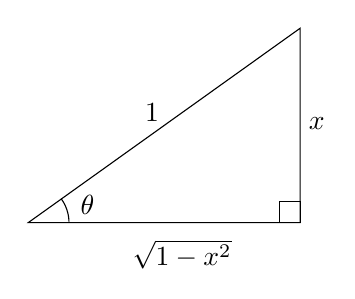
\begin{tikzpicture}[x=0.75pt,y=0.75pt,yscale=-1,xscale=1]
%uncomment if require: \path (0,300); %set diagram left start at 0, and has height of 300

%Shape: Right Triangle [id:dp33900088777115056] 
\draw   (382,83.33) -- (251,177) -- (382,177) -- cycle ;
%Shape: Arc [id:dp14981039391059237] 
\draw  [draw opacity=0] (266.86,165.44) .. controls (269.13,168.55) and (270.51,172.35) .. (270.62,176.48) -- (251,177) -- cycle ; \draw   (266.86,165.44) .. controls (269.13,168.55) and (270.51,172.35) .. (270.62,176.48) ;  
%Shape: Square [id:dp4005119377806101] 
\draw   (372,167) -- (382,167) -- (382,177) -- (372,177) -- cycle ;

% Text Node
\draw (300,184) node [anchor=north west][inner sep=0.75pt]    {$\sqrt{1-x^{2}}$};
% Text Node
\draw (385,125) node [anchor=north west][inner sep=0.75pt]    {$x$};
% Text Node
\draw (306,118.4) node [anchor=north west][inner sep=0.75pt]    {$1$};
% Text Node
\draw (275,162.4) node [anchor=north west][inner sep=0.75pt]    {$\theta $};
\end{tikzpicture}
\end{center}
\mar{Draw the triangles for the other two examples.}
\end{itemize}



